\section{The Motor Circuit}
	
	\subsection{Motor Controller Chips}
		
		\textit{<Written explanation to be added after the workshop>}
		
		%\begin{figure}
		%	\centering
		%	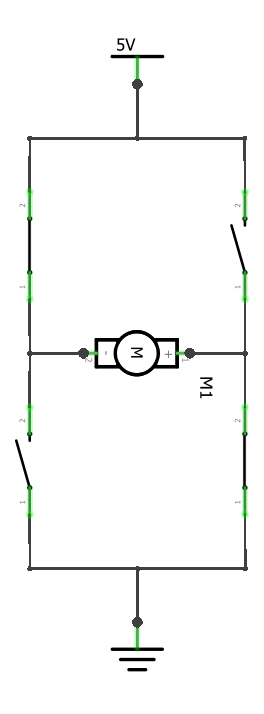
\includegraphics[height=5cm]{sections/2_motor/schematic_HbridgeA}
		%	\hspace{5mm}
		%	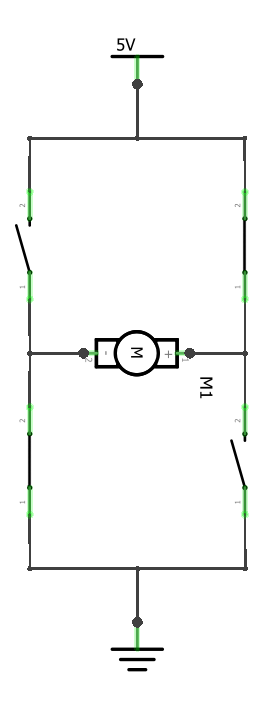
\includegraphics[height=5cm]{sections/2_motor/schematic_HbridgeB}
		%	\caption{A H-bridge circuit in both configurations}
		%	\label{fig:schematic_HbridgeA}
		%\end{figure}

		
		The pinout for the L293D/L239DNE chip is shown in Appendix \autoref{sec:pinoutL293}.

			
	\subsection{Setting up a Motor Circuit}
		
		Firstly, we'll ensure we have the motors and chip powered.
		
		\begin{enumerate}[noitemsep]
			\item Remember to shut down and \textbf{unplug} your Pi first.
			\item \textbf{Place} the L293DNE chip across the central gap, noting the orientation. In the illustration, the semicircle cutout is facing to the right.
			\item \textbf{Connect} both positive buses with a jumper cable to a 5V pin. 
			\item \textbf{Connect} the Motor voltage and Chip voltage pins with their closest positive bus.
			\item \textbf{Connect} at least two ground pins on the chip to the motor's negative bus.
			\item \textbf{Connect} at least two GND pins on the pi to the Motor negative bus.
		\end{enumerate}
		
		Your breadboard should now look like figure \ref{fig:schematic_3}. Now, we will add the GPIO inputs and motor.
		
		\begin{figure}[h]
			\centering
			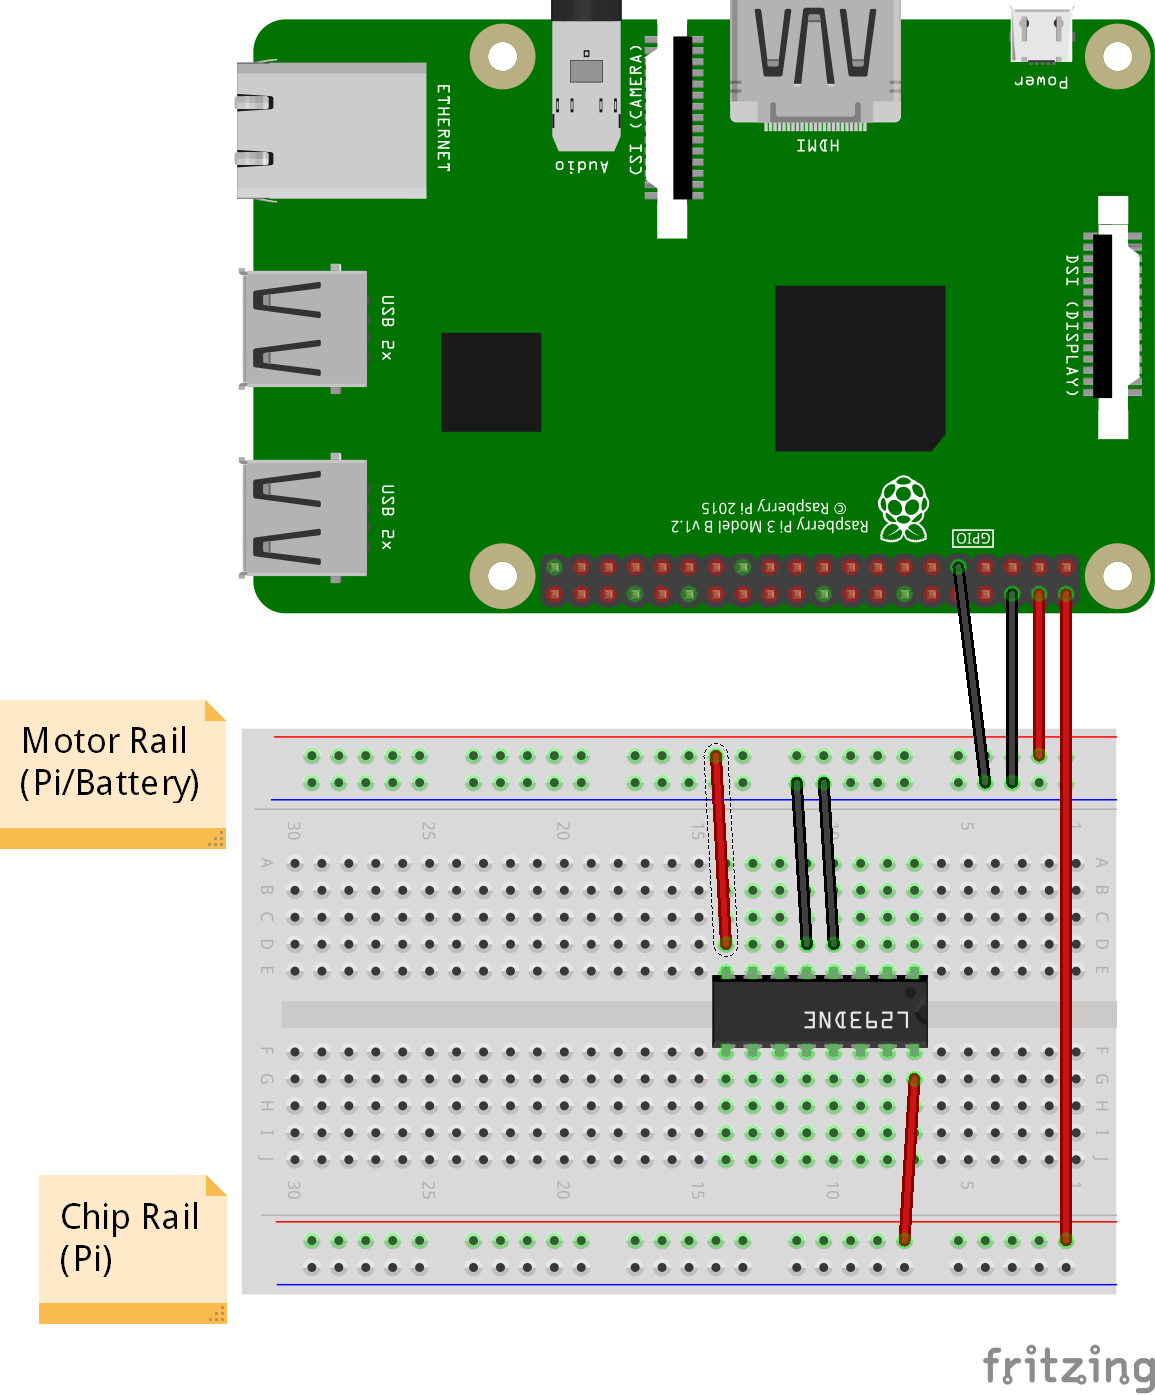
\includegraphics[width=0.6\linewidth]{McrRaspJam/011_Motors/2_motor/schematic_3}
			\caption{Powering the L293DNE.}
			\label{fig:schematic_3}
		\end{figure}
		
		\begin{enumerate}[noitemsep]
			\setcounter{enumi}{6}
			\item \textbf{Connect} GPIO pin 23 to input 2A, and GPIO pin 24 to input 2B with a pair of jumper cables.
			\item \textbf{Connect} GPIO pin 25 to Enable 2 with another cable.
			\item \textbf{Connect} Connect the motor to the two motor pins (on the motor 2 side). \scriptsize \textit{If you don't have crocodile clips, try bending the pins of two jumper cables to keep them in place.} \normalsize
			\item \textbf{Connect} at least two GND pins on the pi to the Motor negative bus.
		\end{enumerate}
		
		If you're happy that your circuit is equivalent to the one shown in figure \ref{fig:schematic_5}, you can try turning on your Pi. If it makes it to the desktop, you probably haven't done anything too disastrous!
		
		\begin{figure}[h]
			\centering
			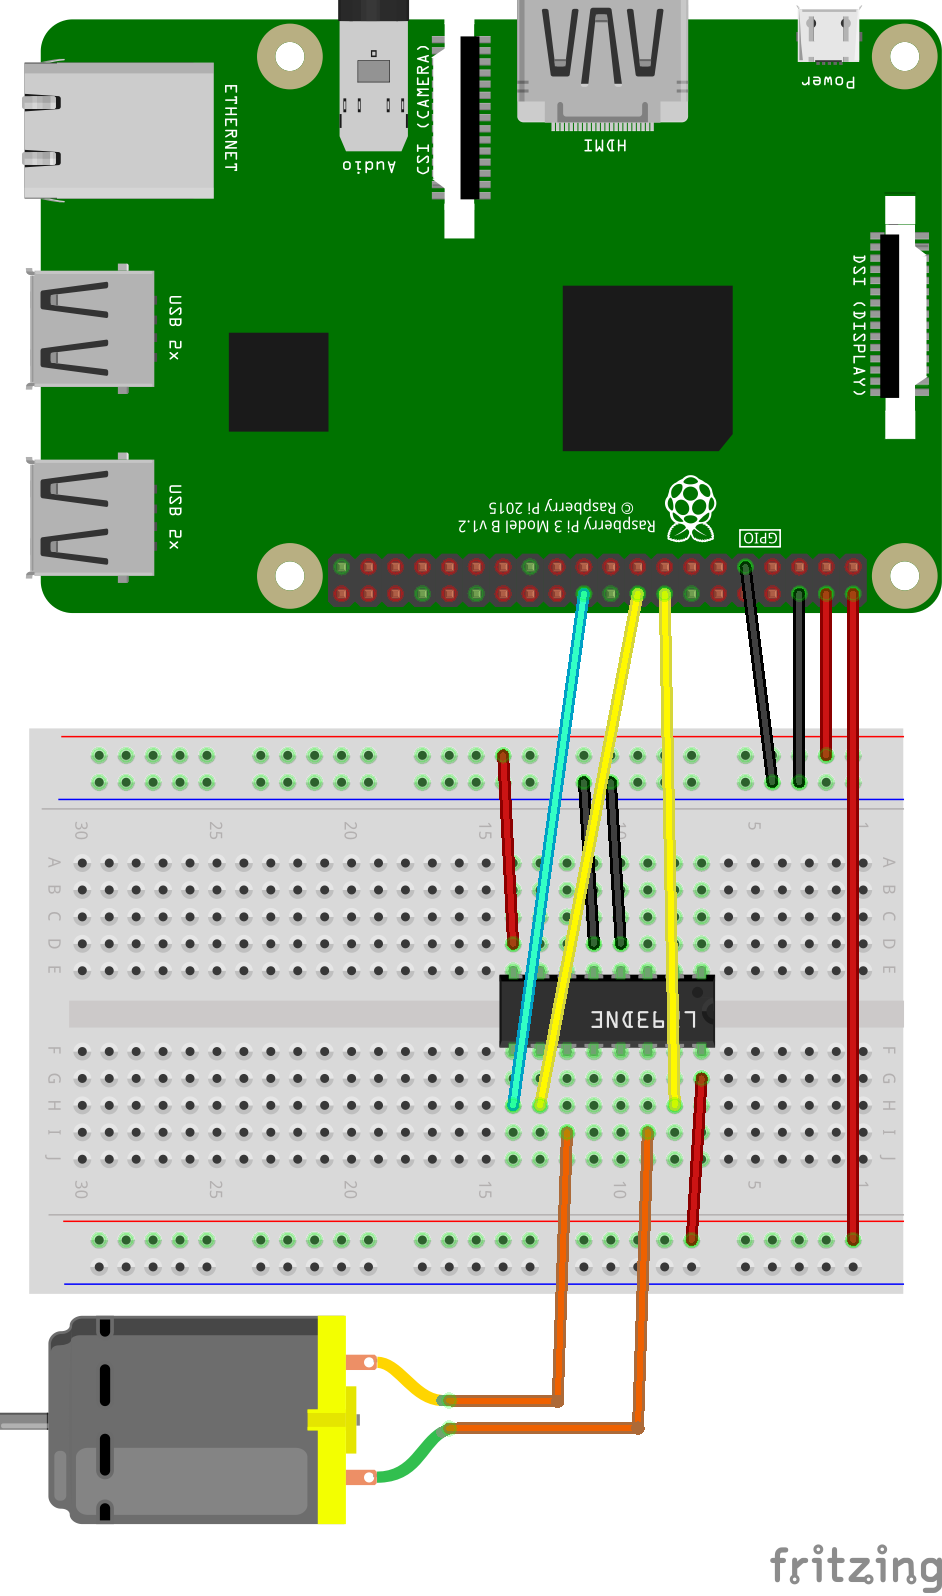
\includegraphics[width=0.6\linewidth]{McrRaspJam/011_Motors/2_motor/schematic_5}
			\caption{The complete motor circuit.}
			\label{fig:schematic_5}
		\end{figure}
		
	\subsection{Programming the Motor}
	
		Start with a copy of the template program from before:
		
		\lstinputlisting[style=Python, lastline=6]{McrRaspJam/011_Motors/2_motor/1_Motor.py}
		
		This time, we will set up all three of the GPIO pins that we connected:
	
		\lstinputlisting[style=Python, firstline=7, firstnumber=7, lastline=15]{McrRaspJam/011_Motors/2_motor/1_Motor.py}
		
		Remember that to turn on a motor, we need to set two opposing signals for A and B, then set enable to high. Therefore, to turn the motor on:
		
		\lstinputlisting[style=Python, firstline=16, firstnumber=16, lastline=20]{McrRaspJam/011_Motors/2_motor/1_Motor.py}
		
		As with our LED, we will leave the motor running for a few seconds before turning it off. We do not need to change the A or B input, we can just change `Enable' to turn off the motor:
		
		\lstinputlisting[style=Python, firstline=21, firstnumber=21, lastline=26]{McrRaspJam/011_Motors/2_motor/1_Motor.py}
		
		After adding the GPIO.cleanup() function, you can now try running your program.
		
		Make sure your motor is connected, and hold onto the body of the motor whilst running the program, as the motor likes to wiggle free of it's wires.
		
		\subsubsection*{Reverse Gear}
		
			One final thing to check. Our motor controller should allow us to run the motor in reverse. 
			
			Make the following changes to your program, and have a go at filling in the missing parameters for the GPIO.output function calls:
					
			\lstinputlisting[style=Python, firstline=21, firstnumber=21, lastline=38]{McrRaspJam/011_Motors/2_motor/2_Motor.py}
			
			It will be difficult to tell which way the motor is spinning with nothing attached, but it tends to make a slightly different noise when running in the other direction.
			
			To double check, you can try placing some Blu Tack on the motor shaft and shaping it to make the spin more obvious.
			
			Congratulations on getting your motor working!
			